%!TEX root = ../tesis.tex
\chapter{Soluci\'on Propuesta}
\label{sec:solucion}


% introduccion
Existen numerosas aplicaciones en el \'area del reconocimiento del habla, cada una de ellas
satisface distintos tipos de requerimientos establecidos por los usuarios finales. En el
cap\'itulo anterior se marc\'o la diferencia en el proceso de dise\~nar interfaces basadas en reconocimiento
del habla y el proceso de implementar interfaces, para una aplicaci\'on determinada, basadas en reconocimiento del habla.

Este cap\'itulo presenta, justifica y eval\'ua la soluci\'on espec\'ifica al problema de implementar una intefaz
basada en reconomiento del habla para una aplicaci\'on determinada.


%!TEX root = ../tesis.tex

\section{Tecnolog\'ia a Utilizar}
\label{sec:tecnologia-utilizada}

Como se expone en la secci\'on~\ref{sec:problema-especifico}, se propone el dise\~no
de una interfaz para componer m\'usica utilizando la voz. Adem\'as, este trabajo 
opta por la metodolog\'ia de trabajo
de c\'odigo abierto, lo cual implica: 

\begin{itemize}
    \item Utilizar tecnolog\'ias de c\'odigo abierto para el desarrollo de la interfaz.
    \item Establecer un proceso de desarrollo transparente y abierto.
    \item Ofrecer la interfaz desarrollada, junto con su c\'odigo fuente, de manera libre 
        y gratuita para la comunidad de c\'odigo abierto.
\end{itemize}

La metodolog\'ia adoptada para implementar la interfaz permite utilizar un proyecto
existente como punto de partida, y as\'i dise\~nar e implementar una interfaz alternativa que permite
controlar la aplicaci\'on por comandos de voz. Adem\'as,
el hecho de incorporar una nueva interfaz, permite analizar
una de las motivaciones de la secci\'on~\ref{sec:motivacion}: un programa de composici\'on
musical, que recibe comandos sonoros y emite tambi\'en un resultado sonoro, podr\'ia ser
m\'as natural para el usuario. 

La interfaz desarrollada se denomina \emph{TamTam Listens} y se basa en tecnolog\'ias de c\'odigo abierto.
Toma como punto de partida la aplicaci\'on \emph{TamTam Edit} y para realizar el reconocimiento 
de comandos de voz utiliza los proyectos \emph{PocketSphinx} \cite{PocketSphinxHomePage} 
y \emph{Voxforge} \cite{Voxforge}.  A continuaci\'on se presentan los proyectos
utilizados como punto de partida para la soluci\'on implementada.

\subsection{TamTam Edit}
\label{sec:tamtam-edit}

La m\'usica es a menudo descrita como la forma m\'as pura de representaci\'on matem\'atica, es m\'as,
te\'oricos de la m\'usica han utilizado las matem\'aticas para resolver problemas musicales
\cite{TheSoundOfNumbers}. Esto sirvi\'o de inspiraci\'on para la creaci\'on del compendio de 
actividades\footnote{Una Actividad, es una aplicaci\'on en el entorno de escritorio \emph{Sugar}.}
conocido como \emph{TamTam} desarrollado para la computadora XO\footnote{La XO, es una computadora 
port\'atil de bajo costo y consumo desarrollada por el proyecto \gls{olpc}.},
con los siguientes objetivos:

\begin{itemize}
    \item Proveer a los ni\~nos un ambiente de informaci\'on cultural construyendo m\'usica y sonidos.
    \item Brindar una experiencia sonora/musical divertida para usuarios sin conocimientos musicales.
    \item Promover un camino hacia experiencias musicales m\'as sofisticadas.
    \item Promover un instrumento musical con su propio ``sonido''.
    \item Desarrollar un ambiente din\'amico y mutable que propone la simpleza y permite la complejidad.
    \item Favorecer la creaci\'on de m\'usica grupalmente.
    \item Introducir los conceptos musicales y otros como: programaci\'on y audio.
\end{itemize}

\emph{TamTam Edit} es una aplicaci\'on, que forma parte del conjunto de actividades musicales 
\emph{TamTam}, que proporciona una interfaz intuitiva para crear, modificar y organizar notas ubicadas 
en pistas virtuales.
Adem\'as incluye una paleta de casi cien tipos de sonidos y modelos de construcci\'on musical que permite 
crear distintos tipos de variaciones en estilos musicales \cite{TamTamWiki}.


Las secciones principales del programa se pueden observar en la figura~\ref{figure:ui-tamtam} 

\begin{figure}[H]
\centering
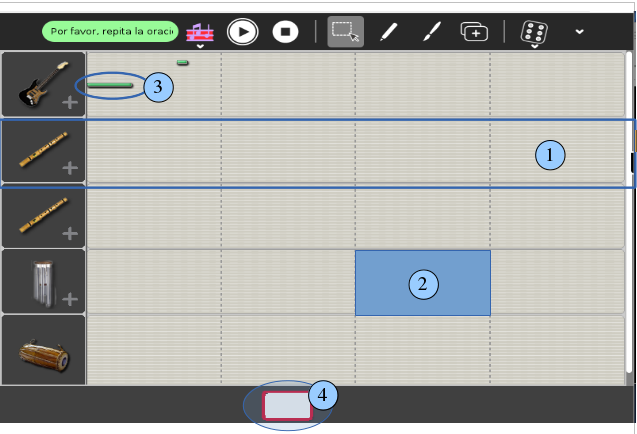
\includegraphics[width=0.8\textwidth]{./graphics/ui-tamtam-edit.png}
\caption{Interfaz de \emph{Tamtam Edit} y sus secciones principales}
\label{figure:ui-tamtam}
\end{figure}

Como se puede apreciar en la figura~\ref{figure:ui-tamtam}, la interfaz se encuentra organizada en 
cinco pistas y cada pista (1) tiene asociada un instrumento (la quinta pista esta reservada para
instrumentos de tipo bater{\'\i}a). Cada pista se divide en 4 
compases (del comp\'as uno al cuatro) y cada comp\'as (2) se divide en 12 tiempos (del uno al doce). 
Las notas (3) se dibujan en los compases, como se puede ver, la longitud de la nota indica su 
duraci\'on y su altura el tipo de nota. Adem\'as la aplicaci\'on esta organizada en partituras (4), que 
son como hojas de cuaderno, y son \'utiles para componer m\'usicas largas.

En general, la interacci\'on entre el usuario y \foreign{TamTam Edit} que se presenta en
la figura~\ref{figure:ui-tamtam} se realiza de modo tradicional.
El usuario utiliza el teclado y el rat\'on para interactuar con la aplicaci\'on a trav\'es de elementos
gr\'aficos como botones y men\'us. 

Este trabajo de grado busca incorporar un medio de interacci\'on alternativo al propuesto por \emph{TamTam Edit}. 
A continuaci\'on se presentan los motivos que determinaron la elecci\'on de esta aplicaci\'on como punto de partida:

\begin{itemize}
    \item Impacto social: \emph{TamTam Edit} es una aplicaci\'on que forma parte de la plataforma establecida
    por el proyecto \gls{olpc}, el cual busca potenciar el proceso educativo \cite{OLPC}. 
    Los ni\~nos con alg\'un tipo de discapacidad tienen a menudo problemas para utilizar una computadora mediante
    dispositivos perif\'ericos tradicionales como el mouse o el teclado.

    En estos casos, la posibilidad de operar esta actividad mediante la voz ser{\'\i}a de gran beneficio 
    para los ni\~nos, mejorando la accesibilidad de la plataforma, y generando por tanto un impacto social
    positivo importante.
    \item Naturalidad de interacci\'on: utilizar la voz para interactuar con una aplicaci\'on podr{\'\i}a
    ofrecer una mayor naturalidad con respecto al enfoque tradicional de interacci\'on, teniendo en cuenta
    que es el medio de interacci\'on entre las personas.
    \item No reinventar la rueda: como el objetivo es incorporar una interfaz basada en reconocimiento del
    habla a una aplicaci\'on, se elige \emph{TamTam Edit} para no construir la aplicaci\'on desde cero,
    sino extender las capacidades de una ya existente.
    \item C\'odigo abierto: el motivo anterior es posible gracias a que \emph{TamTam Edit} es un 
    proyecto de c\'odigo abierto, lo cual brinda a los desarrolladores la libertad de extender las 
    funcionalidades de la aplicaci\'on.
    \item Lenguaje de programaci\'on: la actividad se encuentra implementada en el lenguaje de 
    programaci\'on Python. La librer{\'\i}a de reconocimiento del habla a ser utilizada proporociona 
    \emph{bindings} 
    \footnote{Un \emph{binding} es un componente \emph{software}
   que permite hacer uso de las funcionalidades prove{\'\i}das por una librer{\'\i}a, implementada
    en un determinado lenguaje de programaci\'on, utilizando un lenguaje de programaci\'on diferente. 
    En este caso particular, \emph{Pocketsphinx} est\'a implementado en C y C++.} para 
    este lenguaje, lo cual supone una ventaja importante para la implementaci\'on de la interfaz.
\end{itemize}


\subsection{Voxforge}
\foreign{Voxforge} es un proyecto que busca recopilar grabaciones de voz de modo a crear 
y ofrecer varios corpus de habla bajo una licencia que permita su libre utilizaci\'on. 

A partir de estos corpus, es posible construir modelos ac\'usticos para su uso con motores de 
reconocimiento del habla de c\'odigo abierto, como \foreign{Pocketsphinx}.

\foreign{Voxforge} cuenta con grabaciones en diferentes idiomas, entre ellos ingĺ\'es, franc\'es, 
alem\'an y espa\~nol.


\subsection{PocketSphinx}

El cap\'itulo~\ref{sec:tecnologias} clasifica a las herramientas que permiten implementar soluciones
basadas en reconocimiento del habla en tres categor\'ias: Aplicaciones, \gls{api}s y Librer\'ias. 
Dada la naturaleza de este trabajo, se opta por elegir una librer\'ia para implementar la interfaz
alternativa a la ofrecida por \emph{TamTam Edit}.

Para la implementaci\'on de la interfaz operable a trav\'es de la voz se elige la librer\'ia 
\emph{PocketSphinx} que, como se menciona en la secci\'on~\ref{sec:pocketsphinx}, es un motor de 
reconocimiento del habla orientado a la optimizaci\'on del rendimiento y la portabilidad.

Uno de los objetivos espec\'ificos de este trabajo es aplicar y contrastar en la pr\'actica
los conocimientos te\'oricos adquiridos. Como indica la secci\'on~\ref{sec:librerias}, una librer\'ia es
el tipo de herramienta que requiere un conocimiento t\'ecnico espec\'ifico del \'area, adem\'as de
brindar una alta flexibilidad permitiendo al programador manipular los distintos componentes del
proceso de reconocimiento del habla. Por este motivo, una librer\'ia se considera la herramienta 
m\'as adecuada para cumplir el objetivo mencionado anteriormente.

A continuaci\'on se presentan los motivos t\'ecnicos que determinaron la elecci\'on de esta librer\'ia:

\begin{itemize}
    \item \emph{PocketSphinx} est\'a orientada a la optimizaci\'on del rendimiento, resultando adecuada 
    para sistemas con recursos limitados, como la computadora \emph{XO}.
    \item La librer\'ia es un proyecto de c\'odigo abierto, por lo tanto se cumple la metodolog\'ia 
    de trabajo adoptada.
    \item \emph{PocketSphinx} ofrece soporte \emph{offline}, lo cual permite su utilizaci\'on en ambientes
    sin conexi\'on a internet, como ocurre frecuentemente con las \emph{XO}.
    \item Existen \foreign{bindings} para el lenguaje de programaci\'on Python, lo cual hace muy 
    sencilla la tarea de utilizar la librer\'ia desde el c\'odigo Python.
\end{itemize}

\foreign{PocketSphinx} implementa el proceso del reconocimiento del habla basado en el enfoque 
estad{\'\i}stico, el cual se present\'o en el cap{\'\i}tulo~\ref{sec:proceso}. La librer{\'\i}a incluye
los diferentes algoritmos necesarios para las fases del proceso.

\begin{figure}[H] 
\centering
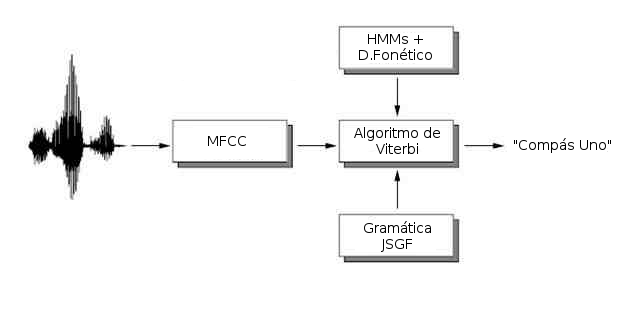
\includegraphics[width=0.8\textwidth]{./graphics/pocketsphinx.png}
\caption{Reconocimiento del habla mediante PocketSphinx. Gr\'afico basado en \cite{VerenichASR}.}
\label{figure:proceso-pocketsphinx}
\end{figure}

Como conjunto de caracter{\'\i}sticas espectrales, \foreign{Pocketsphinx} utiliza los coeficientes
espectrales en las frecuencias de mel (MFCC por sus siglas en ingl\'es).

En los \gls{hmm} del modelo ac\'ustico, utiliza mezclas Gaussianas para definir las probabilidades de 
transici\'on entre estados. El diccionario fon\'etico debe ser definido por el desarrollador.

Aunque \foreign{PocketSphinx} soporta modelos de lenguaje basados en n-gramas, para este trabajo 
se utiliza un modelo de lenguaje basado en gram\'atica. Esto se debe a la simpleza del lenguaje y a la 
falta de datos de entrenamiento para un modelo estad{\'\i}stico del mismo.

Como decodificador se utiliza el algoritmo de Viterbi, haciendo uso de la t\'ecnica de b\'usqueda en haz
para reducir el espacio de b\'usqueda.

\section{M\'etricas de Evaluaci\'on}
\label{sec:metricas}

\section{Resultados Experimentales}
\label{sec:resultados}

